\documentclass[conference]{IEEEtran}

% ============================================================
% Packages
% ============================================================
\usepackage[T1]{fontenc}
\usepackage[utf8]{inputenc}
\usepackage{cite}
\usepackage{amsmath,amssymb}
\usepackage{booktabs}
\usepackage{array}
\usepackage{graphicx}
\usepackage{xcolor}
\usepackage{xurl}
\usepackage{pgfplots}
\usepackage[hidelinks]{hyperref}
\usepackage{stfloats}

\pgfplotsset{compat=1.18}
\usetikzlibrary{patterns,plotmarks}

% ============================================================
% Model and precision macros
% ============================================================
\newcommand{\model}{Qwen2.5-0.5B-Instruct}
\newcommand{\fp}{\texttt{fp32}}
\newcommand{\fphalf}{\texttt{fp16}}
\newcommand{\qfour}{\texttt{q4}}
\newcommand{\qfourhalf}{\texttt{q4f16}}
\newcommand{\mlchalf}{\texttt{q4f16\_1}}
\newcommand{\mlcfull}{\texttt{q4f32\_1}}
\newcommand{\missing}{\bot}

% ============================================================
% Chart colors
% ============================================================
\definecolor{paperblue}{RGB}{0,78,124}
\definecolor{paperorange}{RGB}{194,99,0}
\definecolor{paperteal}{RGB}{0,119,107}
\definecolor{papergray}{RGB}{185,185,185}

% ============================================================
% Shared chart style
% ============================================================
\pgfplotsset{
  paperaxis/.style={
    tick label style={font=\footnotesize},
    label style={font=\footnotesize},
    axis line style={black},
    tick align=outside,
    scaled ticks=false,
    legend style={
      font=\scriptsize,
      draw=none,
      fill=none,
      cells={anchor=west}
    }
  }
}

% ============================================================
% Title and authors (no forced line breaks in title)
% ============================================================
\title{Does Running a Small LLM in the Browser Change Its Answers? A Case Study of Native ONNX and Browser WebGPU Stacks on a Dual-GPU Laptop}

\author{
\IEEEauthorblockN{Sudip Niroula}
\IEEEauthorblockA{
Independent Researcher\\
Nepal
}
\and
\IEEEauthorblockN{Mandip Pokharel}
\IEEEauthorblockA{
Independent Researcher\\
Nepal
}
}

\begin{document}

\maketitle

% ============================================================
% Abstract
% ============================================================
\begin{abstract}
Browser-based language model inference changes the execution
stack, numerical representation, and hardware used to generate
an answer. Aggregate benchmark accuracy does not establish
whether these changes preserve individual outputs. This paper
presents an archived-output case study of
Qwen2.5-0.5B-Instruct using native Node.js ONNX CPU execution
and browser inference through Transformers.js and WebLLM on
a Windows 11 laptop with Intel UHD and NVIDIA GeForce
RTX 2050 graphics. Fourteen saved run files contain
3,920 evaluations of fixed subsets comprising 200 MMLU
questions and 100 GSM8K problems. The analysis separates
task success, parsing coverage, agreement between jointly
parsed answers, and literal text agreement. Matched
requested-dtype comparisons show severe degradation in the
tested Transformers.js WebGPU path: GSM8K task success
decreases from 31\% to 0\%--1\% for fp16 and from 24\%
to 0\% for q4f16. A browser WebAssembly q4 diagnostic instead
matches native q4 text and raw token IDs on all
20 diagnostic items. A scoring audit identifies 39 unparsed
MMLU responses in the native fp32 reference and substantial
dependence on last-number extraction for GSM8K. Direct
comparison of Intel-labelled and NVIDIA-labelled WebLLM runs
finds identical decoded text on all 300 items for q4f32\_1,
compared with 95\% MMLU and 46\% GSM8K text agreement for
q4f16\_1. These observations motivate explicit
deployment-fidelity testing, but do not establish an isolated
browser effect, a diagnosed runtime defect, or cross-device
guarantees.
\end{abstract}

\begin{IEEEkeywords}
browser inference, WebGPU, WebAssembly, small language models,
ONNX Runtime, WebLLM, quantization, output fidelity,
reproducibility
\end{IEEEkeywords}


% ============================================================
\section{Introduction}
\label{sec:introduction}
% ============================================================

Client-side language model inference can avoid per-request
inference-server computation and can keep prompts local when
the application does not transmit them. Transformers.js and
WebLLM provide different software paths for running language
models in browser applications \cite{transformersjs,webllm}.
Their availability makes deployment on consumer hardware
increasingly practical.

Deployment quality, however, is not described completely by
throughput or aggregate benchmark accuracy. A developer may
evaluate a model through a native runtime and later deploy a
browser-compatible representation. The resulting system may
change the weight format, compiler, execution provider,
numerical precision, device, and generation defaults.
A shared model name is therefore insufficient evidence that
the two deployments will produce the same outputs.

Prior work has shown that compression can preserve aggregate
benchmark accuracy while changing which individual answers
are correct \cite{accuracy}. Browser inference research has
also identified numerical precision and hardware
heterogeneity as important implementation concerns
\cite{llamas,maczan}. These observations motivate paired
evaluation: the same questions should be compared item by
item, rather than interpreting similar aggregate scores as
equivalent behaviour.

This study examines \model{} across native ONNX CPU execution
and browser inference through Transformers.js and WebLLM.
The testbed is one consumer laptop with integrated Intel
graphics and a discrete NVIDIA GPU. The analysis is
intentionally scoped as a case study of recorded deployment
configurations, rather than a general comparison of browsers
and native inference.

Three evaluation dimensions are distinguished:

\begin{itemize}
\item \textbf{Task success:} whether an extracted answer
matches the benchmark target, counting missing extractions
as unsuccessful.

\item \textbf{Answer fidelity:} whether two configurations
produce the same extracted answer, separating jointly
parsed answers from shared parsing failures.

\item \textbf{Text fidelity:} whether generated strings are
literally identical, with token-sequence comparisons where
the records support them.
\end{itemize}

These dimensions answer different questions. Two
configurations can reproduce the same incorrect answer.
They can also achieve the same task-success rate while
succeeding on different items. Finally, both can fail to
produce a parsable answer, creating outcome agreement
without a shared substantive answer.


\subsection{Research Questions}

The study addresses four questions:

\begin{itemize}
\item \textbf{RQ1: Matched requested-dtype comparison.}
How do browser Transformers.js WebGPU and WebAssembly
outputs compare with native CPU outputs when the same ONNX
repository identifier and dtype are requested?

\item \textbf{RQ2: Cross-adapter consistency.}
How often do Intel-labelled and NVIDIA-labelled browser runs
on the same host produce identical extracted answers and
decoded text?

\item \textbf{RQ3: Reference fidelity.}
How do native quantized ONNX and browser WebLLM deployments
differ from a native \fp{} reference in task success, answer
agreement, and directional correctness transitions?

\item \textbf{RQ4: Scoring validity.}
How do missing extractions, generation budgets, and
permissive extraction rules affect interpretation of the
observed results?
\end{itemize}


\subsection{Contributions}

The contributions are:

\begin{enumerate}
\item A fixed, item-level evaluation protocol with shared
JavaScript message construction and answer extraction.

\item Direct matched requested-dtype comparisons and direct
cross-adapter comparisons, rather than comparisons only
against aggregate reference accuracy.

\item A scoring audit separating parsing coverage,
conditional answer agreement, correctness transitions,
and literal text agreement.

\item A versioned analysis of 3,920 archived responses,
with explicit provenance and causal limitations.
\end{enumerate}

Correctness flips are not presented as a newly discovered
phenomenon. The contribution is their application, together
with a parsing audit, to the evaluated native and browser
deployment paths.


% ============================================================
\section{Background and Related Work}
\label{sec:related}
% ============================================================

\subsection{Browser Inference Systems and Numerical Validation}

WebLLM provides browser-local inference through a
compiler-based WebGPU execution stack \cite{webllm}.
Transformers.js provides a separate deployment path based on
ONNX Runtime, supporting CPU execution through WebAssembly
and GPU execution through WebGPU \cite{transformersjs}.

These frameworks should not be treated as interchangeable
implementations of an otherwise completely controlled
experiment. They may differ in model representation,
quantization, compilation, tokenization interfaces, and
generation configuration. Comparisons between them can
characterize deployment outcomes without identifying the
causal contribution of each internal component.

\emph{Llamas on the Web} studies memory-efficient,
performance-portable, multi-precision WebGPU inference across
devices and vendors, noting that reduced-precision accumulation
can degrade text coherence in models including Qwen2.5 and
motivating 32-bit accumulation \cite{llamas}. Other recent
studies validate single WebGPU operator numerics against CPU
references across GPU vendors \cite{maczan} or examine
browser-versus-native likelihood fidelity on domain-specific
mixture-of-experts models \cite{genomeocean}. The present work
focuses instead on paired benchmark answers, parsing
behaviour, and decoded-text identity under a fixed consumer
laptop deployment protocol.


\subsection{Compression and Behavioural Fidelity}

Dutta et al.'s \emph{Accuracy is Not All You Need} establishes
that aggregate accuracy can conceal substantial changes in
item-level correctness under compression \cite{accuracy}.
This motivates reporting both directions of correctness
change and distinguishing those changes from wrong-to-wrong
answer differences.

This study adopts that perspective and adds an extraction
distinction. When a reference output does not contain a
parsable answer, a later correct extraction is a
wrong-to-correct task-success transition. It is not
necessarily evidence that a substantive wrong answer became
correct.


\subsection{Model and Benchmark Scope}

The evaluated model belongs to the Qwen2.5 family
\cite{qwen}. Questions are drawn from MMLU \cite{mmlu}
and GSM8K \cite{gsm8k}.

The results apply to fixed subsets under the prompts,
generation limits, and extraction rules used here.
They are not full-benchmark scores and are not directly
comparable with published results using different prompting,
option scoring, or generation protocols.


% ============================================================
\section{Experimental Design}
\label{sec:design}
% ============================================================

\subsection{Evaluation Inventory}

The archive contains fourteen saved run files. Thirteen
contain all 300 questions, while a WebAssembly diagnostic
contains ten questions from each task. One full
NVIDIA-labelled \fphalf{} WebGPU run repeats an earlier
configuration. Thus, the inventory contains 3,920 item
evaluations and 28 task-specific rows, not 28 independent
deployment configurations \cite{archive,repository}.

\begin{table}[t]
\caption{Evaluation Inventory}
\label{tab:inventory}
\centering
\footnotesize
\setlength{\tabcolsep}{5pt}
\begin{tabular}{@{}lrrr@{}}
\toprule
Execution group & Files & Items/file & Total\\
\midrule
Native ONNX CPU & 4 & 300 & 1,200\\
Transformers.js WebGPU & 5 & 300 & 1,500\\
WebLLM WebGPU & 4 & 300 & 1,200\\
Transformers.js WASM & 1 & 20 & 20\\
\midrule
Total & 14 & -- & 3,920\\
\bottomrule
\end{tabular}
\end{table}

The repeat file is retained in descriptive reporting but
excluded from the family of pairwise significance tests.
The small WebAssembly diagnostic is also excluded from
that family.


\subsection{Hardware and Software}

All inference runs were conducted on one Windows laptop.
Table~\ref{tab:environment} summarizes the recorded
inference and analysis environments \cite{repository}.

\begin{table}[t]
\caption{Recorded Inference and Analysis Environment}
\label{tab:environment}
\centering
\footnotesize
\begin{tabular}{@{}
p{0.31\columnwidth}
p{0.62\columnwidth}
@{}}
\toprule
Component & Recorded configuration\\
\midrule
Operating system & Windows 11, 64-bit\\
CPU & Intel Core i5-13420H (8C/12T)\\
System memory & 8 GB RAM\\
Integrated graphics & Intel UHD Graphics, Gen-12LP\\
Discrete graphics &
NVIDIA GeForce RTX 2050 Laptop GPU, 4 GB GDDR6\\
Browser & Chrome user-agent reporting 139.0.0.0\\
Native host & Node.js v20+\\
Transformers.js & 4.3.0\\
WebLLM & 0.2.85\\
Analysis environment & Python 3.14.2, SciPy 1.18.1, Transformers 5.17.0\\
\bottomrule
\end{tabular}
\end{table}

A single host reduces differences in host CPU, installed
memory, and operating environment. It does not eliminate
execution-stack differences or provide replication across
independent machines.

The Chrome version is reported as recorded, rather than as
an independently verified complete build identifier.
The archive similarly records Node.js only at the stated
version granularity.


\subsection{Execution Configurations}

Native runs use Transformers.js through the ONNX Runtime
Node.js CPU path. Four dtypes are requested from
\path{onnx-community/Qwen2.5-0.5B-Instruct}:
\fp{}, \fphalf{}, \qfour{}, and \qfourhalf{}.

Browser Transformers.js runs use the WebGPU path for
\fphalf{} and \qfourhalf{} under both adapter labels.
The WebAssembly diagnostic uses \qfour{} on the CPU.

Browser WebLLM runs use the \mlchalf{} and \mlcfull{}
precompiled builds. In the MLC quantization registry,
these builds differ in their \texttt{float16} and
\texttt{float32} \texttt{model\_dtype} settings \cite{mlc}.
They do not constitute an accumulation-only intervention.

Throughout this paper, a dtype identifies the requested
model representation. It does not establish the precision
of every intermediate computation or native CPU instruction.


\subsection{Adapter Labelling}

Chrome was assigned to the power-saving or high-performance
graphics preference in Windows. The browser page recorded
adapter information using a main-page
\path{navigator.gpu.requestAdapter()} call
\cite{repository}.

This is evidence about the page-visible adapter after the
preference change, not direct attestation of the internal
adapter handle selected by every inference worker.
Consequently, the terms \emph{Intel-labelled} and
\emph{NVIDIA-labelled} are used for the saved browser runs.

The WebAssembly diagnostic executes on the CPU.
An available GPU recorded in page metadata does not make it
a GPU inference run.


\subsection{Historical Artifact Provenance}

The native and browser Transformers.js runners request the
same repository identifier and dtype strings. However,
historical ONNX revisions and file checksums were not pinned
across inference dates \cite{repository}.

The comparison therefore establishes matched requested
identifiers, not verified byte-for-byte identity of every
historically downloaded model artifact. This distinction is
retained in the interpretation of RQ1.


\subsection{Questions and Generation Protocol}

The fixed evaluation file contains 200 MMLU questions and
100 GSM8K problems, sampled with seed 2026. The MMLU subset
covers all 57 subjects: 34 subjects contribute four
questions, 18 contribute three, and five contribute two
\cite{repository}.

Both runners import \path{site/harness.js} for message
construction and answer extraction. The system message is:

\begin{quote}
\small
You are Qwen, created by Alibaba Cloud.
You are a helpful assistant.
\end{quote}

MMLU generation is limited to five new tokens.
GSM8K generation is limited to 320 new tokens.
Sampling was disabled (\texttt{do\_sample = false}) in
Transformers.js, and WebLLM used temperature zero and seed
zero \cite{repository}.

These settings remove intentional sampling variation.
They do not guarantee identical outputs across hardware,
implementations, or sessions.

The shared harness controls application-level message
construction. It does not by itself prove that every
framework renders identical internal prompt token sequences
or applies identical generation defaults.


% ============================================================
\section{Evaluation and Statistical Methods}
\label{sec:methods}
% ============================================================

\subsection{Archived Extraction Rules}

The archived MMLU extractor first searches for a standalone
uppercase A--D letter. If unsuccessful, it falls back to an
uppercase A--D character without a word-boundary requirement.
The fallback can therefore match a character inside a word
\cite{repository}.

The GSM8K extractor searches for an
\texttt{answer is <number>} pattern and otherwise returns the
last number in the output. Such a number can be a final
answer or an intermediate calculation in an incomplete
response.

The historical predictions and correctness flags are
preserved. Additional extraction audits are reported
separately rather than silently replacing the original
scores.


\subsection{Task Success and Parsing Coverage}

For item $i$, let $g_i$ denote the target and $a_i$
the extracted answer. A missing extraction is denoted by
$\missing$. Task success is

\begin{equation}
S =
\frac{1}{N}
\sum_{i=1}^{N}
\mathbf{1}\{a_i\neq\missing \land a_i=g_i\}.
\label{eq:success}
\end{equation}

Parse rate is

\begin{equation}
P =
\frac{1}{N}
\sum_{i=1}^{N}
\mathbf{1}\{a_i\neq\missing\}.
\label{eq:parse}
\end{equation}

Accuracy among parsed responses divides the number of
correct answers by the number of nonmissing extractions.
It is diagnostic, not an unbiased replacement for task
success, because configurations can produce parsable
answers on different subsets.

A strict-extraction audit requires a standalone uppercase
A--D letter (\texttt{r"\textbackslash b([ABCD])\textbackslash b"})
for MMLU and a restrictive explicit marker match
(\texttt{r"answer is\textbackslash s*([\textbackslash -0-9,\textbackslash .]+)"})
for GSM8K. Strict parse rate (\texttt{strict\_parse\_rate})
measures extraction coverage under this restrictive regex;
strict-extraction accuracy (\texttt{strict\_acc}) also
requires the extracted answer to match the target.

These stricter rules do not guarantee that an extraction
is the intended final answer. A standalone letter can occur
in explanatory text, while an explicit numeric answer can
still be incorrect.


\subsection{Answer Agreement}

For reference answer $r_i$ and test answer $t_i$,
define the jointly parsed set

\begin{equation}
B = \{i:r_i\neq\missing \land t_i\neq\missing\}.
\label{eq:both}
\end{equation}

Valid-answer agreement is

\begin{equation}
A_{\mathrm{valid}} =
\frac{
\sum_{i\in B}\mathbf{1}\{r_i=t_i\}
}{
|B|
}.
\label{eq:valid}
\end{equation}

It is undefined when $|B|=0$.
All-outcome agreement is

\begin{equation}
A_{\mathrm{all}} =
\frac{1}{N}
\sum_{i=1}^{N}
\mathbf{1}\{r_i=t_i\},
\label{eq:all}
\end{equation}

where two missing extractions count as equal outcomes.

Numerators and denominators are reported explicitly when
space permits. High valid-answer agreement on a very small
jointly parsed subset is not evidence of broad fidelity.


\subsection{Correctness Transitions}

Let $N_{\mathrm{c2w}}$ count items on which the reference
succeeds and the test configuration does not.
Let $N_{\mathrm{w2c}}$ count the opposite transition.
Missing answers are unsuccessful under these definitions.

The net change in task success is

\begin{equation}
\Delta S =
\frac{
N_{\mathrm{w2c}}-N_{\mathrm{c2w}}
}{N},
\label{eq:delta}
\end{equation}

whereas the correctness-flip rate is

\begin{equation}
F =
\frac{
N_{\mathrm{w2c}}+N_{\mathrm{c2w}}
}{N}.
\label{eq:flip}
\end{equation}

The analysis additionally identifies transitions involving
a missing reference or test extraction
(\texttt{unparsed\_ref\_to\_correct} and
\texttt{correct\_to\_unparsed\_test}).
These transitions remain part of task success but should
not all be described as substantive answer reversals.


\subsection{Text and Token Fidelity}

Exact text agreement compares literal decoded strings
without whitespace trimming. Raw generated token IDs are
compared across all paired items when both records contain
them.

When raw IDs are unavailable, strings are retokenized using
the \path{Qwen/Qwen2.5-0.5B-Instruct} tokenizer explicitly
loaded at pinned revision:

\begin{quote}
\footnotesize
\path{7ae557604adf67be50417f59c2c2f167def9a775}
\end{quote}

The loaded \path{tokenizer.json} artifact has SHA-256
checksum
\path{c0382117ea329cdf097041132f6d735924b697924d6f6fc3945713e96ce87539}
\cite{repository}.

The first divergent token is the first unequal position,
or the shorter sequence length when one sequence is a
strict prefix of the other. The sample median is calculated
over divergent sequences.

Raw-token divergence and retokenized-text divergence are
not interchangeable. Retokenization cannot recover every
detail of original generation, including special tokens
removed during decoding.


\subsection{Token-Cap Indicators}

For runs containing raw output IDs, token-cap indicators
use the stored sequence length. For WebLLM records without
those IDs, they use retokenized output length
\cite{repository}.

Reaching the nominal generation cap is not identical to a
verified truncation finish reason. Retokenized lengths are
also not exact reconstructions of the original generation
length. The paper therefore reports cap indicators,
not exact counts of unfinished solutions.


\subsection{Statistical Analysis}

Paired task-success differences are evaluated using a
two-sided exact binomial McNemar test, implemented through
SciPy's binomial test \cite{scipy,scipybinom}.

For $b=N_{\mathrm{c2w}}$, $c=N_{\mathrm{w2c}}$, and
$m=b+c>0$, the test evaluates discordant outcomes under a
binomial null with probability $1/2$. When $m=0$, the
comparison has $p=1$.

Holm's step-down correction is applied to 22 comparisons
against native \fp{}, excluding reference rows, the repeat
file, and the WebAssembly diagnostic
\cite{holm,repository}.

All-outcome agreement intervals use 2,000 percentile
bootstrap resamples with seed zero. These intervals describe
item-resampling variation under the fixed protocol,
not uncertainty across hardware, drivers, or sessions.
Degenerate intervals at complete or zero observed agreement
do not establish population certainty.

All inferential results are exploratory because the study
uses small, structured benchmark subsets and lacks
independent host-level replication.


% ============================================================
\section{Results}
\label{sec:results}
% ============================================================

\subsection{MMLU Parsing Changes the Interpretation}
\label{sec:mmluparsing}

The native \fp{} reference succeeds on 78 of 200 MMLU items
and leaves 39 unparsed (38 saturating the five-token limit
and one terminating early at three tokens with the option text
\texttt{WEP} plus EOS on item \texttt{mmlu-1554}). Native
\qfour{} and \qfourhalf{} obtain higher task-success scores
while producing fewer unparsed outputs. WebLLM configurations
also have higher parsing coverage than the reference
\cite{repository}.

\begin{table*}[t]
\caption{
MMLU Task Success and Parsing Audit.
Each Configuration Contains 200 Items.
Conditional Accuracy Uses Each Configuration's Own
Parsed Subset. Strict Parse Rate Equals Permissive Parse
Rate for All Native and WebLLM Rows Shown Here.
}
\label{tab:mmluparsing}
\centering
\footnotesize
\setlength{\tabcolsep}{6pt}
\begin{tabular}{@{}lrrrrr@{}}
\toprule
Configuration &
Correct &
Unparsed &
Parse rate (\%) &
Task success (\%) &
Correct among parsed\\
\midrule
Native fp32 &
78 & 39 & 80.5 & 39.0 &
78/161 = 48.45\%\\

Native fp16 &
76 & 40 & 80.0 & 38.0 &
76/160 = 47.50\%\\

Native q4 &
91 & 14 & 93.0 & 45.5 &
91/186 = 48.92\%\\

Native q4f16 &
93 & 15 & 92.5 & 46.5 &
93/185 = 50.27\%\\

WebLLM q4f16\_1, Intel-labelled &
84 & 1 & 99.5 & 42.0 &
84/199 = 42.21\%\\

WebLLM q4f16\_1, NVIDIA-labelled &
86 & 0 & 100.0 & 43.0 &
86/200 = 43.00\%\\

WebLLM q4f32\_1, Intel-labelled &
89 & 6 & 97.0 & 44.5 &
89/194 = 45.88\%\\

WebLLM q4f32\_1, NVIDIA-labelled &
89 & 6 & 97.0 & 44.5 &
89/194 = 45.88\%\\
\bottomrule
\end{tabular}
\end{table*}

Figure~\ref{fig:mmluoutcomes} separates correct, parsed
incorrect, and unparsed outcomes. It illustrates why higher
task success should not automatically be interpreted as
improved underlying knowledge.


% ============================================================
% FIGURE 1
% ============================================================
\begin{figure}[t]
\centering

\resizebox{\columnwidth}{!}{%
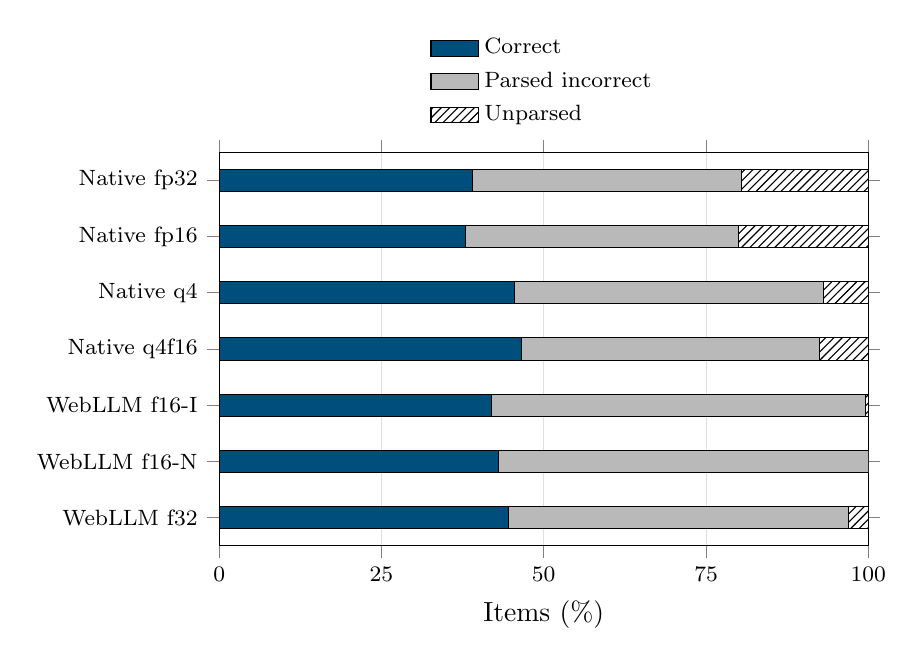
\begin{tikzpicture}
\begin{axis}[
  paperaxis,
  scale only axis=true,
  width=0.68\columnwidth,
  height=5.0cm,
  xbar stacked,
  bar width=8pt,
  xmin=0,
  xmax=100,
  ymin=0.5,
  ymax=7.5,
  xtick={0,25,50,75,100},
  ytick={1,2,3,4,5,6,7},
  y dir=reverse,
  yticklabels={
    Native fp32,
    Native fp16,
    Native q4,
    Native q4f16,
    WebLLM f16-I,
    WebLLM f16-N,
    WebLLM f32
  },
  xlabel={Items (\%)},
  yticklabel style={
    font=\footnotesize,
    align=right
  },
  axis lines=box,
  xmajorgrids=true,
  ymajorgrids=false,
  grid style={
    draw=gray!25,
    line width=0.3pt
  },
  legend style={
    at={(0.5,1.04)},
    anchor=south,
    legend columns=1,
    font=\footnotesize,
    draw=none,
    fill=none,
    cells={anchor=west},
    row sep=1pt
  }
]

% Correct.
\addplot[
  fill=paperblue,
  draw=black,
  line width=0.3pt,
  forget plot
] coordinates {
  (39.0,1)
  (38.0,2)
  (45.5,3)
  (46.5,4)
  (42.0,5)
  (43.0,6)
  (44.5,7)
};

% Parsed but incorrect.
\addplot[
  fill=papergray,
  draw=black,
  line width=0.3pt,
  forget plot
] coordinates {
  (41.5,1)
  (42.0,2)
  (47.5,3)
  (46.0,4)
  (57.5,5)
  (57.0,6)
  (52.5,7)
};

% Unparsed.
\addplot[
  fill=white,
  draw=black,
  line width=0.3pt,
  pattern=north east lines,
  pattern color=black,
  forget plot
] coordinates {
  (19.5,1)
  (20.0,2)
  (7.0,3)
  (7.5,4)
  (0.5,5)
  (0.0,6)
  (3.0,7)
};

\addlegendimage{
  area legend,
  fill=paperblue,
  draw=black
}
\addlegendentry{Correct}

\addlegendimage{
  area legend,
  fill=papergray,
  draw=black
}
\addlegendentry{Parsed incorrect}

\addlegendimage{
  area legend,
  fill=white,
  draw=black,
  pattern=north east lines,
  pattern color=black
}
\addlegendentry{Unparsed}

\end{axis}
\end{tikzpicture}%
}

\caption{
MMLU outcome decomposition under the five-token generation
budget ($N=200$ per configuration).
WebLLM f16-I and f16-N denote the Intel-labelled and
NVIDIA-labelled \mlchalf{} runs, respectively.
WebLLM f32 represents the identical outcome counts of the
two \mlcfull{} runs.
Data are from the pinned parsing export \cite{repository}.
}
\label{fig:mmluoutcomes}
\end{figure}


Native \qfourhalf{} has 25 wrong-to-correct transitions
relative to \fp{}, but eight originate from missing \fp{}
answers. The corresponding counts are 11 of 29 for
Intel-labelled WebLLM \mlchalf{}, 12 of 30 for its
NVIDIA-labelled counterpart, and 10 of 30 for each \mlcfull{}
run \cite{repository}.

Shared missing answers affect agreement as well.
Native \fphalf{} and \fp{} match on 196 of 200 outcomes,
but 39 matches are shared parsing failures.
Agreement among jointly parsed answers is 157/160,
or 98.12\%.

The five-token protocol therefore measures a mixture of
answer correctness, formatting behaviour, and budget
sensitivity. The audit identifies this confound; it does
not quantify the counterfactual score under a longer
generation budget.


\subsection{GSM8K Scores Depend on Extraction Policy}
\label{sec:gsmparsing}

All native and WebLLM configurations produce a number under
the archived GSM8K extractor. Explicit-marker extraction
succeeds on very few outputs, however.
Native \fp{} and \fphalf{} have no explicit-marker matches
despite archived task-success scores of 29\% and 31\%,
respectively \cite{repository}.

\begin{table*}[t]
\caption{
GSM8K Extraction Sensitivity and Token-Cap Indicators.
Each Configuration Contains 100 Items.
Marker Parsed Counts Matches to the Restrictive Explicit-Marker
Regex (\texttt{strict\_parse\_rate}); Marker Correct
(\texttt{strict\_acc}) Also Requires the Extracted Number to
Match the Target.
}
\label{tab:gsmparsing}
\centering
\footnotesize
\setlength{\tabcolsep}{5pt}
\begin{tabular}{@{}lrrrrrl@{}}
\toprule
Configuration &
Archived correct &
Archived parsed &
Marker parsed &
Marker correct &
At cap &
Length source\\
\midrule
Native fp32 &
29 & 100 & 0 & 0 & 44 &
Raw token IDs\\

Native fp16 &
31 & 100 & 0 & 0 & 41 &
Raw token IDs\\

Native q4 &
20 & 100 & 3 & 1 & 50 &
Raw token IDs\\

Native q4f16 &
24 & 100 & 3 & 1 & 50 &
Raw token IDs\\

WebLLM q4f16\_1, Intel-labelled &
16 & 100 & 0 & 0 & 50 &
Retokenized text\\

WebLLM q4f16\_1, NVIDIA-labelled &
19 & 100 & 0 & 0 & 49 &
Retokenized text\\

WebLLM q4f32\_1, Intel-labelled &
18 & 100 & 2 & 1 & 45 &
Retokenized text\\

WebLLM q4f32\_1, NVIDIA-labelled &
18 & 100 & 2 & 1 & 45 &
Retokenized text\\
\bottomrule
\end{tabular}
\end{table*}

The archived scores consequently depend heavily on
last-number fallback extraction.
The strict audit measures extraction-policy sensitivity,
not whether every response without an explicit marker is
mathematically incorrect.

The cap indicators likewise should not be interpreted as
verified unfinished solutions.
Without consistently recorded finish reasons, the
distinction between completed and budget-limited generation
remains imperfect.


\subsection{Matched Requested-Dtype Comparisons}
\label{sec:matched}

The browser WebAssembly \qfour{} diagnostic matches native
CPU \qfour{} in decoded text and raw token IDs on all twenty
diagnostic items. Their task-success rates on those same
items are 20\% for MMLU and 40\% for GSM8K
\cite{repository}.

In contrast, the tested \fphalf{} and \qfourhalf{} WebGPU
runs show severe degradation relative to native runs with
the same requested dtype (Tables~\ref{tab:matched_outcomes}
and~\ref{tab:matched_fidelity}).

\begin{table*}[t]
\caption{
Direct Matched Requested-Dtype Comparisons (Task and Answer Outcomes).
Native and Browser Values Use the Same Item IDs.
The NVIDIA fp16 Repeat Has the Same Reported Scores as Its
First Run and Is Omitted Here for Brevity.
}
\label{tab:matched_outcomes}
\centering
\footnotesize
\setlength{\tabcolsep}{6pt}
\begin{tabular}{@{}llrrrrr@{}}
\toprule
Browser configuration & Task & $N$ & Native success (\%) & Browser success (\%) & Valid agreement & All-outcome agreement\\
\midrule
WASM q4 diagnostic & MMLU & 10 & 20.0 & 20.0 & 8/8 (100.00\%) & 10/10 (100.00\%)\\
WASM q4 diagnostic & GSM8K & 10 & 40.0 & 40.0 & 10/10 (100.00\%) & 10/10 (100.00\%)\\
\midrule
TJS WebGPU fp16, Intel-labelled & MMLU & 200 & 38.0 & 5.5 & 13/43 (30.23\%) & 42/200 (21.00\%)\\
TJS WebGPU fp16, NVIDIA-labelled & MMLU & 200 & 38.0 & 7.0 & 11/45 (24.44\%) & 42/200 (21.00\%)\\
TJS WebGPU fp16, Intel-labelled & GSM8K & 100 & 31.0 & 0.0 & 0/56 (0.00\%) & 0/100 (0.00\%)\\
TJS WebGPU fp16, NVIDIA-labelled & GSM8K & 100 & 31.0 & 1.0 & 0/51 (0.00\%) & 0/100 (0.00\%)\\
\midrule
TJS WebGPU q4f16, Intel-labelled & MMLU & 200 & 46.5 & 2.5 & 3/17 (17.65\%) & 17/200 (8.50\%)\\
TJS WebGPU q4f16, NVIDIA-labelled & MMLU & 200 & 46.5 & 2.0 & 1/16 (6.25\%) & 16/200 (8.00\%)\\
TJS WebGPU q4f16, Intel-labelled & GSM8K & 100 & 24.0 & 0.0 & 0/4 (0.00\%) & 0/100 (0.00\%)\\
TJS WebGPU q4f16, NVIDIA-labelled & GSM8K & 100 & 24.0 & 0.0 & 1/5 (20.00\%) & 1/100 (1.00\%)\\
\bottomrule
\end{tabular}
\end{table*}

\begin{table*}[t]
\caption{
Direct Matched Requested-Dtype Comparisons (Generation Fidelity Against Matched-Dtype Native Controls).
Exact Text and Exact Raw Token Matches Are Reported as Counts Alongside Token-Level Divergence Statistics.
}
\label{tab:matched_fidelity}
\centering
\footnotesize
\setlength{\tabcolsep}{6pt}
\begin{tabular}{@{}llrrrrrr@{}}
\toprule
Browser configuration & Task & $N$ & Exact text & Exact token IDs & Median div.\ token & Div.\ at token 0 & Div.\ at token 1\\
\midrule
WASM q4 diagnostic & MMLU & 10 & 10/10 & 10/10 & -- & 0/10 & 0/10\\
WASM q4 diagnostic & GSM8K & 10 & 10/10 & 10/10 & -- & 0/10 & 0/10\\
\midrule
TJS WebGPU fp16, Intel-labelled & MMLU & 200 & 0/200 & 0/200 & 0 & 196/200 & 3/200\\
TJS WebGPU fp16, NVIDIA-labelled & MMLU & 200 & 1/200 & 1/200 & 0 & 196/200 & 2/200\\
TJS WebGPU fp16, Intel-labelled & GSM8K & 100 & 0/100 & 0/100 & 0 & 87/100 & 4/100\\
TJS WebGPU fp16, NVIDIA-labelled & GSM8K & 100 & 0/100 & 0/100 & 0 & 82/100 & 8/100\\
\midrule
TJS WebGPU q4f16, Intel-labelled & MMLU & 200 & 1/200 & 1/200 & 0 & 193/200 & 6/200\\
TJS WebGPU q4f16, NVIDIA-labelled & MMLU & 200 & 0/200 & 0/200 & 0 & 193/200 & 7/200\\
TJS WebGPU q4f16, Intel-labelled & GSM8K & 100 & 0/100 & 0/100 & 0 & 100/100 & 0/100\\
TJS WebGPU q4f16, NVIDIA-labelled & GSM8K & 100 & 0/100 & 0/100 & 0 & 100/100 & 0/100\\
\bottomrule
\end{tabular}
\end{table*}

Figure~\ref{fig:matchedgsm} visualizes the GSM8K contrast.
The zero-valued WebGPU measurements are explicitly marked
at the baseline so that measured zero success cannot be
mistaken for missing data.

Because the model identifiers were not historically
checksum-pinned, the finding is stated as a discrepancy
under matched requested identifiers rather than identical
verified model bytes.


% ============================================================
% FIGURE 2
% ============================================================
\begin{figure}[t]
\centering

\resizebox{\columnwidth}{!}{%
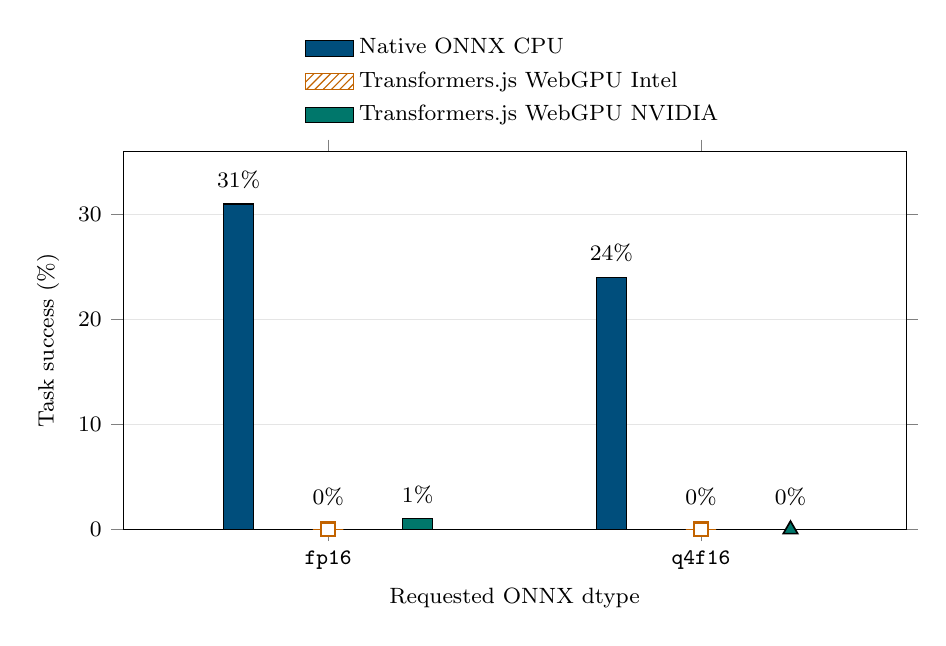
\begin{tikzpicture}
\begin{axis}[
  paperaxis,
  scale only axis=true,
  width=0.82\columnwidth,
  height=4.8cm,
  xmin=0.45,
  xmax=2.55,
  ymin=0,
  ymax=36,
  xtick={1,2},
  xticklabels={
    \texttt{fp16},
    \texttt{q4f16}
  },
  ytick={0,10,20,30},
  xlabel={Requested ONNX dtype},
  ylabel={Task success (\%)},
  ymajorgrids=true,
  xmajorgrids=false,
  grid style={gray!20},
  clip=false,
  legend style={
    at={(0.5,1.04)},
    anchor=south,
    legend columns=1,
    font=\footnotesize,
    draw=none,
    fill=none,
    cells={anchor=west},
    row sep=1pt
  }
]

% Native CPU.
\addplot[
  ybar,
  bar width=11pt,
  bar shift=0pt,
  fill=paperblue,
  draw=black,
  forget plot
] coordinates {
  (0.76,31)
  (1.76,24)
};

% Intel-labelled WebGPU.
\addplot[
  ybar,
  bar width=11pt,
  bar shift=0pt,
  fill=white,
  draw=paperorange,
  pattern=north east lines,
  pattern color=paperorange,
  forget plot
] coordinates {
  (1.00,0)
  (2.00,0)
};

% NVIDIA-labelled WebGPU.
\addplot[
  ybar,
  bar width=11pt,
  bar shift=0pt,
  fill=paperteal,
  draw=black,
  forget plot
] coordinates {
  (1.24,1)
  (2.24,0)
};

% Intel zero markers at the true y=0 coordinate.
\addplot[
  only marks,
  mark=square*,
  mark size=2.5pt,
  mark options={
    draw=paperorange,
    fill=white,
    line width=0.8pt
  },
  forget plot
] coordinates {
  (1.00,0)
  (2.00,0)
};

% NVIDIA zero marker at the true y=0 coordinate.
\addplot[
  only marks,
  mark=triangle*,
  mark size=3pt,
  mark options={
    draw=black,
    fill=paperteal,
    line width=0.6pt
  },
  forget plot
] coordinates {
  (2.24,0)
};

% Explicit percentage labels.
\node[
  anchor=south,
  font=\footnotesize,
  yshift=2pt
] at (axis cs:0.76,31) {31\%};

\node[
  anchor=south,
  font=\footnotesize,
  yshift=2pt
] at (axis cs:1.76,24) {24\%};

\node[
  anchor=south,
  font=\footnotesize,
  yshift=5pt
] at (axis cs:1.00,0) {0\%};

\node[
  anchor=south,
  font=\footnotesize,
  yshift=5pt
] at (axis cs:2.00,0) {0\%};

\node[
  anchor=south,
  font=\footnotesize,
  yshift=2pt
] at (axis cs:1.24,1) {1\%};

\node[
  anchor=south,
  font=\footnotesize,
  yshift=5pt
] at (axis cs:2.24,0) {0\%};

% Explicit legend swatches.
\addlegendimage{
  area legend,
  fill=paperblue,
  draw=black
}
\addlegendentry{Native ONNX CPU}

\addlegendimage{
  area legend,
  fill=white,
  draw=paperorange,
  pattern=north east lines,
  pattern color=paperorange
}
\addlegendentry{Transformers.js WebGPU Intel}

\addlegendimage{
  area legend,
  fill=paperteal,
  draw=black
}
\addlegendentry{Transformers.js WebGPU NVIDIA}

\end{axis}
\end{tikzpicture}%
}

\caption{
GSM8K task success in matched requested-dtype comparisons
($N=100$ per run), using the archived permissive extraction
rules. Intel and NVIDIA denote the adapter-labelled runs.
Baseline markers and 0\% labels represent measured zero
task success, not missing observations.
The figure compares Transformers.js WebGPU with native
ONNX CPU execution; it does not show WebLLM results
\cite{repository}.
}
\label{fig:matchedgsm}
\end{figure}


Relative to matched native \fphalf{}, the Intel-labelled and
NVIDIA-labelled WebGPU \fphalf{} outputs diverge at the first
raw generated token on 87/100 and 82/100 GSM8K items,
respectively (Table~\ref{tab:matched_fidelity}). Relative to
matched native \qfourhalf{}, both \qfourhalf{} WebGPU runs
diverge at token zero on all 100 GSM8K items (whereas
relative to native \fp{} in Appendix~\ref{app:complete},
99 of 100 items diverge at token zero and 1 item diverges
at token one) \cite{repository}.

The WebAssembly diagnostic supports successful end-to-end
parity for its configuration and subset.
It does not isolate which component accounts for the \fphalf{}
or \qfourhalf{} WebGPU discrepancy. Possible distinctions
include graph processing, operator execution, cache handling,
runtime versions, and generation behaviour.
The logs do not diagnose one of these as the cause.


\subsection{Direct Cross-Adapter Comparisons}
\label{sec:cross}

WebLLM \mlcfull{} produces identical decoded text across the
two labelled runs on all 300 items.
WebLLM \mlchalf{} instead matches on 190/200 MMLU strings and
46/100 GSM8K strings (Table~\ref{tab:cross})
\cite{repository}.

\begin{table*}[t]
\caption{
Direct Intel-Labelled Versus NVIDIA-Labelled Comparisons.
MMLU Contains 200 Items and GSM8K Contains 100.
All-Outcome Agreement Includes Shared Missing Answers.
}
\label{tab:cross}
\centering
\footnotesize
\setlength{\tabcolsep}{6pt}
\begin{tabular}{@{}llrrrrr@{}}
\toprule
Browser build &
Task &
Intel success (\%) &
NVIDIA success (\%) &
Valid agreement &
All-outcome agreement &
Exact text\\
\midrule
WebLLM q4f16\_1 &
MMLU & 42.0 & 43.0 &
194/199 (97.49\%) & 194/200 (97.00\%) & 190/200 (95.00\%)\\

WebLLM q4f16\_1 &
GSM8K & 16.0 & 19.0 &
59/100 (59.00\%) & 59/100 (59.00\%) & 46/100 (46.00\%)\\

WebLLM q4f32\_1 &
MMLU & 44.5 & 44.5 &
194/194 (100.00\%) & 200/200 (100.00\%) & 200/200 (100.00\%)\\

WebLLM q4f32\_1 &
GSM8K & 18.0 & 18.0 &
100/100 (100.00\%) & 100/100 (100.00\%) & 100/100 (100.00\%)\\
\midrule
Transformers.js fp16 &
MMLU & 5.5 & 7.0 &
37/41 (90.24\%) & 170/200 (85.00\%) & 128/200 (64.00\%)\\

Transformers.js fp16 &
GSM8K & 0.0 & 1.0 &
24/42 (57.14\%) & 59/100 (59.00\%) & 27/100 (27.00\%)\\

Transformers.js q4f16 &
MMLU & 2.5 & 2.0 &
11/12 (91.67\%) & 189/200 (94.50\%) & 140/200 (70.00\%)\\

Transformers.js q4f16 &
GSM8K & 0.0 & 0.0 &
3/3 (100.00\%) & 97/100 (97.00\%) & 36/100 (36.00\%)\\
\bottomrule
\end{tabular}
\end{table*}

Figure~\ref{fig:crosswebllm} shows the text-agreement result.
It establishes consistency of decoded outputs for this
dataset and labelled pair.
It does not establish an accumulation-only mechanism or a
guarantee across devices.


% ============================================================
% FIGURE 3
% ============================================================
\begin{figure}[t]
\centering

\resizebox{\columnwidth}{!}{%
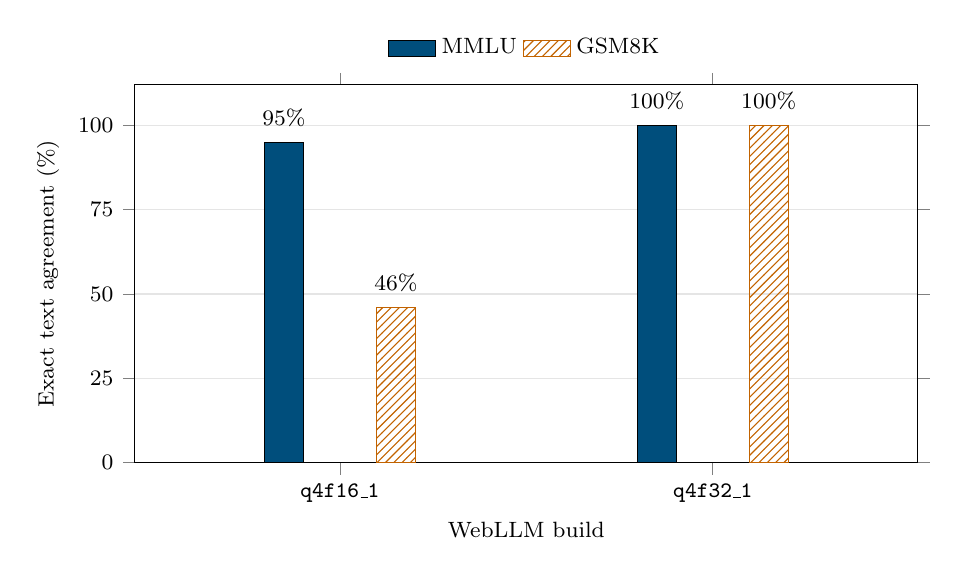
\begin{tikzpicture}
\begin{axis}[
  paperaxis,
  scale only axis=true,
  width=0.82\columnwidth,
  height=4.8cm,
  xmin=0.45,
  xmax=2.55,
  ymin=0,
  ymax=112,
  ytick={0,25,50,75,100},
  xtick={1,2},
  xticklabels={
    \texttt{q4f16\_1},
    \texttt{q4f32\_1}
  },
  xlabel={WebLLM build},
  ylabel={Exact text agreement (\%)},
  ymajorgrids=true,
  xmajorgrids=false,
  grid style={gray!20},
  clip=false,
  legend style={
    at={(0.5,1.04)},
    anchor=south,
    legend columns=2,
    font=\footnotesize,
    draw=none,
    fill=none,
    cells={anchor=west}
  }
]

% MMLU.
\addplot[
  ybar,
  bar width=14pt,
  bar shift=0pt,
  fill=paperblue,
  draw=black,
  forget plot
] coordinates {
  (0.85,95)
  (1.85,100)
};

% GSM8K.
\addplot[
  ybar,
  bar width=14pt,
  bar shift=0pt,
  fill=white,
  draw=paperorange,
  pattern=north east lines,
  pattern color=paperorange,
  forget plot
] coordinates {
  (1.15,46)
  (2.15,100)
};

\node[
  anchor=south,
  font=\footnotesize,
  yshift=2pt
] at (axis cs:0.85,95) {95\%};

\node[
  anchor=south,
  font=\footnotesize,
  yshift=2pt
] at (axis cs:1.15,46) {46\%};

\node[
  anchor=south,
  font=\footnotesize,
  yshift=2pt
] at (axis cs:1.85,100) {100\%};

\node[
  anchor=south,
  font=\footnotesize,
  yshift=2pt
] at (axis cs:2.15,100) {100\%};

\addlegendimage{
  area legend,
  fill=paperblue,
  draw=black
}
\addlegendentry{MMLU}

\addlegendimage{
  area legend,
  fill=white,
  draw=paperorange,
  pattern=north east lines,
  pattern color=paperorange
}
\addlegendentry{GSM8K}

\end{axis}
\end{tikzpicture}%
}

\caption{
Direct decoded-text agreement between Intel-labelled and
NVIDIA-labelled WebLLM runs.
MMLU uses 200 paired items and GSM8K uses 100.
Complete observed agreement is limited to these recorded
outputs \cite{repository}.
}
\label{fig:crosswebllm}
\end{figure}


The Transformers.js \qfourhalf{} GSM8K comparison demonstrates
a different issue. Both runs have zero task success but 97\%
all-outcome agreement.
Their valid-answer agreement is based on only three jointly
parsed items.
Agreement without parsing coverage and task success would
therefore be misleading.


\subsection{Comparison Against Native FP32}
\label{sec:reference}

The complete paired comparisons are provided in
Appendix~\ref{app:complete}.

Native \qfour{} and \qfourhalf{} each have 35 MMLU correctness
transitions, or 17.5\% of all items.
WebLLM \mlchalf{} has 52 transitions, or 26.0\%, while
\mlcfull{} has 49, or 24.5\% \cite{repository}.

These rates include parsing-related transitions.
Nevertheless, answer turnover remains after restricting
comparison to jointly parsed responses.
Native \qfour{} and \qfourhalf{} each agree with \fp{} on
121/161 parsed pairs, or 75.16\%.
WebLLM configurations agree on 61.49\%--64.60\% of jointly
parsed pairs.

The result supports the established distinction between
net accuracy change and item-level fidelity
\cite{accuracy}.
It does not imply that every departure from \fp{} is harmful:
\fp{} is a reference configuration rather than a
ground-truth model.


\subsection{Statistical Interpretation}
\label{sec:statistics}

After Holm correction across 22 comparisons (reported in
Appendix~\ref{app:holm}), the eight non-repeat Transformers.js
WebGPU task comparisons against \fp{} remain significant at
the family-wise 0.05 threshold. None of the native quantized
or WebLLM comparisons remains significant under that
correction \cite{repository}.

For example, the WebLLM \mlcfull{} GSM8K comparison has an
unadjusted $p$-value of 0.0266 and a Holm-adjusted $p$-value
of 0.3192.

A non-significant correctness test does not establish
output equivalence.
On MMLU, \mlcfull{} agrees with \fp{} on only 104/161 jointly
parsed answers despite a non-significant net task-success
difference.

These tests assess paired correctness, not equality of
strings, model distributions, or reasoning processes.


\subsection{Initialization and Repeatability}

The diagnostic notes report \fp{} WebGPU initialization
failures with \texttt{ERROR\_CODE: 6} and
\texttt{std::bad\_alloc} under both selected graphics
preferences \cite{repository}.

The available logs do not isolate host-memory allocation,
WebAssembly heap allocation, GPU buffers, or another loader
component.
The observation establishes an initialization failure of
this configuration, not a universal inability to run \fp{}
models in browsers.

The saved NVIDIA-labelled \fphalf{} WebGPU repeat reproduces
the reported task-success scores and directional flip
counts.
This supports repeatability of the observed outcome under
the repeated configuration, not universal determinism
across sessions.


% ============================================================
\section{Discussion}
\label{sec:discussion}
% ============================================================

\subsection{Consistency and Correctness Are Different}

The results distinguish two deployment properties.

First, WebLLM \mlcfull{} is fully consistent across the two
labelled runs in decoded text on the tested items,
but differs substantially from native \fp{}.

Second, degraded Transformers.js configurations can agree
on failed outcomes while achieving little or no task
success.
A fidelity claim therefore needs both an explicit reference
and a description of the compared outcome.

``Consistent across the two browser runs'' is different
from ``faithful to native \fp{}.''
Neither statement alone establishes answer quality.


\subsection{What the Runtime Comparison Establishes}

The matched requested-dtype comparisons provide evidence
of a large deployment-path discrepancy.
It appears under both adapter labels and affects both task
success and generation sequences.

However, moving from native CPU to browser WebGPU changes
the execution provider and device, may change runtime builds
and graph-processing paths, and lacks historical model
checksums.
The evidence does not isolate the browser environment as
the causal variable.

A root-cause investigation would require a smaller failing
example, stronger artifact provenance, controlled
prompt-token comparisons, and intermediate or fixed-prefix
numerical validation.
Those experiments are outside the present archived-output
analysis.


\subsection{Interpreting the WebLLM Build Comparison}

The \mlcfull{} build shows stronger observed cross-adapter
text consistency than \mlchalf{}.
This gives a practical reason to evaluate both builds when
consistency matters.

It does not demonstrate that accumulation precision alone
caused the result.
The builds differ in model dtype and compiled numerical
behaviour \cite{mlc}.
The study also does not evaluate their latency, memory,
energy, or throughput trade-offs.

Thus, \mlcfull{} is a candidate for validation, not a universal
deployment recommendation.


\subsection{Scoring Is Part of the System}

The five-token MMLU limit mixes knowledge assessment with
brevity and format compliance.
The GSM8K fallback introduces a different ambiguity:
a numeric prediction can originate from an intermediate
calculation instead of an explicit final answer.

A stronger follow-up protocol should retain the original
scoring for historical comparison while adding:

\begin{itemize}
\item longer MMLU generation with separately reported
parse rates;

\item option-score evaluation where comparable scores
are available;

\item GSM8K finish reasons and explicit final-answer
extraction;

\item manual review of a predefined sample of fallback
extractions;

\item fixed-prefix or teacher-forced numerical comparisons
where logits are accessible.
\end{itemize}

These additions would help distinguish formatting,
incomplete generation, numerical differences, and
substantive answer changes.


% ============================================================
\section{Threats to Validity}
\label{sec:limitations}
% ============================================================

\subsection{Internal Validity}

Historical model hashes are missing.
Matching requested identifiers does not establish identical
downloaded bytes.
The shared harness does not prove identical framework-level
prompt tokenization, and page-level adapter metadata does
not attest to each worker's selected device.

The twenty-item \qfour{} WebAssembly check is not a complete
browser CPU baseline for \fphalf{} or \qfourhalf{}.
ONNX-to-WebLLM comparisons also change quantization,
representation, compiler, runtime, and execution device
together.

These limitations restrict causal attribution, even where
the observed output discrepancy is large.


\subsection{Construct Validity}

Task success depends on prompts, generation budgets, and
extraction rules.
The \fp{} configuration is a reference, not a correctness
oracle.

Literal text identity is deliberately strict.
Harmless wording or whitespace changes can reduce text
agreement without reducing usefulness.
Conversely, extracted-answer agreement can conceal
different reasoning or malformed generation.

Conditional agreement and conditional accuracy are also
selection-sensitive because each configuration can produce
valid answers on a different subset.


\subsection{Statistical Validity}

The main tasks contain only 200 and 100 items.
Most configurations have one saved run, preventing reliable
estimation of session-to-session variation.
The structured MMLU subset is not a simple population-wide
sample.

Holm correction addresses the specified family of
correctness tests.
It does not compensate for absent host-level replication
or make this exploratory case study confirmatory.


\subsection{External Validity}

The study evaluates one small model on one laptop,
one recorded browser environment, and two adapter labels.

Findings should not be generalized to larger models,
mobile hardware, other operating systems, other browser
engines, or later software versions without additional
experiments.

In particular, the severe WebGPU degradation is a result
for the tested path, not a permanent property of browser
inference.


% ============================================================
\section{Reproducibility and Data Availability}
\label{sec:reproducibility}
% ============================================================

The original benchmark archive containing the unmodified
initial evaluation harness and all fourteen raw output JSON
files is permanently archived as version 1.0.0 on Zenodo at
DOI
\href{https://doi.org/10.5281/zenodo.23760946}
{10.5281/zenodo.23760946}
\cite{archive}.
The updated static-audit analysis pipeline, pinned tokenizer
configuration, and five exported CSV summary tables are
archived as version 1.1.0 on Zenodo at DOI
\href{https://doi.org/10.5281/zenodo.23828643}
{10.5281/zenodo.23828643}
and in the GitHub repository \cite{repository}.

The exact Git commit corresponding to version 1.1.0 and used
to generate all reported tables is:

\begin{quote}
\footnotesize
\path{f2e35b70009a23e25e72caa63c64494b4395b461}
\end{quote}

The principal analysis command is:

\begin{quote}
\small\ttfamily
python analyze.py results native-node-cpu/fp32
\end{quote}

The repository and version 1.1.0 archive export primary
comparisons, parsing audits, matched-runtime comparisons,
cross-adapter comparisons, and Holm-adjusted tests.
The tokenizer revision is explicitly pinned in the
analysis \cite{repository}.

This paper reports analysis of archived outputs.
It does not claim that a new independent set of inference
runs was performed during manuscript preparation.

Future replications should additionally record model-file
checksums, exact dependency artifacts, browser build,
graphics-driver versions, worker-level adapter details,
prompt token IDs, generation parameters, and finish reasons.

% ============================================================
\section{Practical Implications}
\label{sec:implications}
% ============================================================

Deployment testing should evaluate the actual target stack
rather than treating successful native execution as
sufficient validation of a browser configuration.

A practical validation suite should report task success,
parse rate, jointly parsed answer agreement, shared missing
outcomes, directional correctness transitions, and text
agreement separately.
A fixed canary set can detect severe regressions but should
complement, rather than replace, larger task evaluation.

For applications prioritizing cross-adapter consistency,
\mlcfull{} is a reasonable candidate to test alongside
\mlchalf{}.
The present finding supports that testing decision,
not a guarantee for other devices or workloads.

Finally, allocation failures should be described at the
level actually observed.
An undiagnosed initialization error does not establish a
universal browser memory limit or make quantization
universally mandatory.


% ============================================================
\section{Conclusion}
\label{sec:conclusion}
% ============================================================

This case study examines output fidelity across native
ONNX CPU and browser inference stacks using fixed benchmark
items on a dual-GPU consumer laptop.

The archived results show severe degradation in the tested
Transformers.js WebGPU path relative to matched
requested-dtype native controls, alongside complete text
and raw-token parity in a twenty-item browser WebAssembly
\qfour{} diagnostic.

They also show that aggregate task-success scores conceal
substantial item-level turnover.
Interpretation requires separating valid-answer disagreement
from parsing changes and acknowledging the dependence of
GSM8K results on fallback extraction.

Direct cross-adapter comparison finds identical decoded
text on all 300 items for WebLLM \mlcfull{}, whereas
\mlchalf{} differs on ten MMLU and fifty-four GSM8K outputs.
This is a scoped empirical consistency result, not an
accumulation-only causal finding or a cross-device guarantee.

The methodological implication is that deployment fidelity
should be measured directly, with an explicit reference and
transparent scoring rules, rather than inferred from model
identifiers or aggregate benchmark accuracy.


% ============================================================
\section*{Author Contributions}
% ============================================================

Sudip Niroula: conceptualization, methodology, software,
evaluation-harness design, audit-pipeline development,
formal analysis, and manuscript drafting and revision.

Mandip Pokharel: hardware configuration, execution of native
and browser benchmark runs, data curation, and output
validation.


% ============================================================
% Appendices 
% ============================================================
\appendices

\section{Complete FP32 Reference Comparisons}
\label{app:complete}

Tables~\ref{tab:complete_outcomes}
and~\ref{tab:complete_transitions} report all 28 task rows
against the native \fp{} reference. The WebAssembly diagnostic
is compared with \fp{} only on its corresponding ten items per
task.

C2W and W2C include transitions involving missing extractions,
with transitions from an unparsed reference response to a
correct test response (\texttt{unparsed\_ref\_to\_correct})
and from a correct reference response to an unparsed test
response (\texttt{correct\_to\_unparsed\_test}) listed
explicitly in Table~\ref{tab:complete_transitions}. The
$p$-values in Table~\ref{tab:complete_outcomes} are
unadjusted.

\begin{table*}[!t]
\caption{
Complete Paired Comparison Against Native FP32 (Answer Outcomes and Parsing).
MMLU Rows Have $N=200$ and GSM8K Rows Have $N=100$,
Except WASM Diagnostic Rows, Which Have $N=10$.
I and N Denote Intel-Labelled and NVIDIA-Labelled Runs.
All Values Are From the Pinned Analysis Export
\cite{repository}.
}
\label{tab:complete_outcomes}
\centering
\small
\setlength{\tabcolsep}{6pt}
\begin{tabular}{@{}llrrrrr@{}}
\toprule
Configuration & Task & Success (\%) & Parse rate (\%) & Valid agreement & All-outcome agreement [95\% CI] & Unadjusted $p$\\
\midrule
Native fp32 & MMLU & 39.0 & 80.5 & 161/161 (100.00\%) & 200/200 (100.00\%) [1.000, 1.000] & 1.0000\\
Native fp16 & MMLU & 38.0 & 80.0 & 157/160 (98.12\%) & 196/200 (98.00\%) [0.960, 0.995] & 0.5000\\
Native q4 & MMLU & 45.5 & 93.0 & 121/161 (75.16\%) & 135/200 (67.50\%) [0.610, 0.735] & 0.0410\\
Native q4f16 & MMLU & 46.5 & 92.5 & 121/161 (75.16\%) & 136/200 (68.00\%) [0.615, 0.740] & 0.0167\\
WASM q4 diagnostic & MMLU & 20.0 & 80.0 & 2/7 (28.57\%) & 4/10 (40.00\%) [0.100, 0.700] & 1.0000\\
TJS WebGPU fp16 I & MMLU & 5.5 & 27.0 & 13/43 (30.23\%) & 41/200 (20.50\%) [0.155, 0.260] & $<10^{-4}$\\
TJS WebGPU fp16 N & MMLU & 7.0 & 27.0 & 11/46 (23.91\%) & 42/200 (21.00\%) [0.155, 0.270] & $<10^{-4}$\\
TJS WebGPU fp16 N rep & MMLU & 7.0 & 27.0 & 11/46 (23.91\%) & 42/200 (21.00\%) [0.155, 0.270] & $<10^{-4}$\\
TJS WebGPU q4f16 I & MMLU & 2.5 & 9.0 & 5/14 (35.71\%) & 40/200 (20.00\%) [0.150, 0.260] & $<10^{-4}$\\
TJS WebGPU q4f16 N & MMLU & 2.0 & 8.0 & 2/13 (15.38\%) & 38/200 (19.00\%) [0.140, 0.250] & $<10^{-4}$\\
WebLLM q4f16\_1 I & MMLU & 42.0 & 99.5 & 99/161 (61.49\%) & 100/200 (50.00\%) [0.430, 0.570] & 0.4885\\
WebLLM q4f16\_1 N & MMLU & 43.0 & 100.0 & 100/161 (62.11\%) & 100/200 (50.00\%) [0.430, 0.570] & 0.3317\\
WebLLM q4f32\_1 I & MMLU & 44.5 & 97.0 & 104/161 (64.60\%) & 110/200 (55.00\%) [0.480, 0.620] & 0.1524\\
WebLLM q4f32\_1 N & MMLU & 44.5 & 97.0 & 104/161 (64.60\%) & 110/200 (55.00\%) [0.480, 0.620] & 0.1524\\
\midrule
Native fp32 & GSM8K & 29.0 & 100.0 & 100/100 (100.00\%) & 100/100 (100.00\%) [1.000, 1.000] & 1.0000\\
Native fp16 & GSM8K & 31.0 & 100.0 & 74/100 (74.00\%) & 74/100 (74.00\%) [0.650, 0.820] & 0.6875\\
Native q4 & GSM8K & 20.0 & 100.0 & 19/100 (19.00\%) & 19/100 (19.00\%) [0.120, 0.270] & 0.0490\\
Native q4f16 & GSM8K & 24.0 & 100.0 & 23/100 (23.00\%) & 23/100 (23.00\%) [0.150, 0.320] & 0.3018\\
WASM q4 diagnostic & GSM8K & 40.0 & 100.0 & 2/10 (20.00\%) & 2/10 (20.00\%) [0.000, 0.500] & 1.0000\\
TJS WebGPU fp16 I & GSM8K & 0.0 & 56.0 & 3/56 (5.36\%) & 3/100 (3.00\%) [0.000, 0.070] & $<10^{-4}$\\
TJS WebGPU fp16 N & GSM8K & 1.0 & 51.0 & 2/51 (3.92\%) & 2/100 (2.00\%) [0.000, 0.050] & $<10^{-4}$\\
TJS WebGPU fp16 N rep & GSM8K & 1.0 & 51.0 & 2/51 (3.92\%) & 2/100 (2.00\%) [0.000, 0.050] & $<10^{-4}$\\
TJS WebGPU q4f16 I & GSM8K & 0.0 & 4.0 & 0/4 (0.00\%) & 0/100 (0.00\%) [0.000, 0.000] & $<10^{-4}$\\
TJS WebGPU q4f16 N & GSM8K & 0.0 & 5.0 & 0/5 (0.00\%) & 0/100 (0.00\%) [0.000, 0.000] & $<10^{-4}$\\
WebLLM q4f16\_1 I & GSM8K & 16.0 & 100.0 & 15/100 (15.00\%) & 15/100 (15.00\%) [0.080, 0.220] & 0.0146\\
WebLLM q4f16\_1 N & GSM8K & 19.0 & 100.0 & 19/100 (19.00\%) & 19/100 (19.00\%) [0.120, 0.270] & 0.0525\\
WebLLM q4f32\_1 I & GSM8K & 18.0 & 100.0 & 20/100 (20.00\%) & 20/100 (20.00\%) [0.120, 0.290] & 0.0266\\
WebLLM q4f32\_1 N & GSM8K & 18.0 & 100.0 & 20/100 (20.00\%) & 20/100 (20.00\%) [0.120, 0.290] & 0.0266\\
\bottomrule
\end{tabular}
\end{table*}

\begin{table*}[!t]
\caption{
Complete Paired Comparison Against Native FP32 (Transitions and Generation Fidelity).
Token Divergence Uses Raw Token IDs for Native and Transformers.js Runs and Retokenized Text for WebLLM Runs \cite{repository}.
}
\label{tab:complete_transitions}
\centering
\small
\setlength{\tabcolsep}{6pt}
\begin{tabular}{@{}llrrrrr@{}}
\toprule
Configuration & Task & C2W / W2C & Unparsed ref$\to$C / C$\to$Unparsed test & Exact text & Med.\ div.\ tok. & Div@0 / Div@1\\
\midrule
Native fp32 & MMLU & 0 / 0 & 0 / 0 & 200/200 & -- & 0 / 0\\
Native fp16 & MMLU & 2 / 0 & 0 / 0 & 182/200 & 1 & 5 / 12\\
Native q4 & MMLU & 11 / 24 & 7 / 0 & 97/200 & 0 & 66 / 29\\
Native q4f16 & MMLU & 10 / 25 & 8 / 0 & 95/200 & 0 & 65 / 32\\
WASM q4 diagnostic & MMLU & 1 / 0 & 0 / 0 & 3/10 & 0 & 6 / 1\\
TJS WebGPU fp16 I & MMLU & 73 / 6 & 2 / 56 & 0/200 & 0 & 196 / 2\\
TJS WebGPU fp16 N & MMLU & 72 / 8 & 3 / 56 & 1/200 & 0 & 196 / 2\\
TJS WebGPU fp16 N rep & MMLU & 72 / 8 & 3 / 56 & 1/200 & 0 & 196 / 2\\
TJS WebGPU q4f16 I & MMLU & 77 / 4 & 1 / 75 & 2/200 & 0 & 179 / 18\\
TJS WebGPU q4f16 N & MMLU & 78 / 4 & 0 / 74 & 0/200 & 0 & 180 / 19\\
WebLLM q4f16\_1 I & MMLU & 23 / 29 & 11 / 0 & 70/200 & 0 & 100 / 24\\
WebLLM q4f16\_1 N & MMLU & 22 / 30 & 12 / 0 & 69/200 & 0 & 100 / 28\\
WebLLM q4f32\_1 I & MMLU & 19 / 30 & 10 / 0 & 74/200 & 0 & 91 / 30\\
WebLLM q4f32\_1 N & MMLU & 19 / 30 & 10 / 0 & 74/200 & 0 & 91 / 30\\
\midrule
Native fp32 & GSM8K & 0 / 0 & 0 / 0 & 100/100 & -- & 0 / 0\\
Native fp16 & GSM8K & 2 / 4 & 0 / 0 & 54/100 & 84.5 & 0 / 3\\
Native q4 & GSM8K & 13 / 4 & 0 / 0 & 0/100 & 0 & 72 / 5\\
Native q4f16 & GSM8K & 10 / 5 & 0 / 0 & 0/100 & 0 & 74 / 7\\
WASM q4 diagnostic & GSM8K & 2 / 2 & 0 / 0 & 0/10 & 0 & 8 / 1\\
TJS WebGPU fp16 I & GSM8K & 29 / 0 & 0 / 12 & 0/100 & 0 & 87 / 4\\
TJS WebGPU fp16 N & GSM8K & 29 / 1 & 0 / 15 & 0/100 & 0 & 82 / 8\\
TJS WebGPU fp16 N rep & GSM8K & 29 / 1 & 0 / 15 & 0/100 & 0 & 82 / 8\\
TJS WebGPU q4f16 I & GSM8K & 29 / 0 & 0 / 26 & 0/100 & 0 & 99 / 1\\
TJS WebGPU q4f16 N & GSM8K & 29 / 0 & 0 / 27 & 0/100 & 0 & 99 / 1\\
WebLLM q4f16\_1 I & GSM8K & 19 / 6 & 0 / 0 & 0/100 & 1 & 0 / 69\\
WebLLM q4f16\_1 N & GSM8K & 16 / 6 & 0 / 0 & 0/100 & 1 & 0 / 69\\
WebLLM q4f32\_1 I & GSM8K & 16 / 5 & 0 / 0 & 0/100 & 1 & 0 / 70\\
WebLLM q4f32\_1 N & GSM8K & 16 / 5 & 0 / 0 & 0/100 & 1 & 0 / 70\\
\bottomrule
\end{tabular}
\end{table*}

\section{Holm Step-Down Multiple-Testing Correction}
\label{app:holm}

Table~\ref{tab:holm} reports the 22-hypothesis Holm step-down
multiple-testing correction across the 11 full experimental
configurations and two benchmark tasks compared against
\texttt{native-node-cpu/fp32} (excluding the reference rows,
the repeat run, and the 20-item WASM diagnostic check).

\begin{table*}[!t]
\caption{
Holm Step-Down Multiple-Testing Correction Across 22 Primary
Hypotheses Against Native FP32.
I and N Denote Intel-Labelled and NVIDIA-Labelled Runs
\cite{repository}.
}
\label{tab:holm}
\centering
\small
\setlength{\tabcolsep}{6pt}
\begin{tabular}{@{}lllrrrl@{}}
\toprule
Configuration &
Task &
Discordant flips &
Unadjusted $p$ &
Holm rank &
Holm-adjusted $p$ &
Significant at $\alpha = 0.05$\\
\midrule
TJS WebGPU q4f16 N & MMLU & c2w=78, w2c=4 & $7.614297\times 10^{-19}$ & 1 & $1.675145\times 10^{-17}$ & Yes\\
TJS WebGPU q4f16 I & MMLU & c2w=77, w2c=4 & $1.449536\times 10^{-18}$ & 2 & $3.044026\times 10^{-17}$ & Yes\\
TJS WebGPU fp16 I & MMLU & c2w=73, w2c=6 & $9.995152\times 10^{-16}$ & 3 & $1.999030\times 10^{-14}$ & Yes\\
TJS WebGPU fp16 N & MMLU & c2w=72, w2c=8 & $5.375096\times 10^{-14}$ & 4 & $1.021268\times 10^{-12}$ & Yes\\
TJS WebGPU fp16 I & GSM8K & c2w=29, w2c=0 & $3.725290\times 10^{-9}$ & 5 & $6.705523\times 10^{-8}$ & Yes\\
TJS WebGPU q4f16 I & GSM8K & c2w=29, w2c=0 & $3.725290\times 10^{-9}$ & 6 & $6.705523\times 10^{-8}$ & Yes\\
TJS WebGPU q4f16 N & GSM8K & c2w=29, w2c=0 & $3.725290\times 10^{-9}$ & 7 & $6.705523\times 10^{-8}$ & Yes\\
TJS WebGPU fp16 N & GSM8K & c2w=29, w2c=1 & $5.774200\times 10^{-8}$ & 8 & $8.661300\times 10^{-7}$ & Yes\\
WebLLM q4f16\_1 I & GSM8K & c2w=19, w2c=6 & 0.0146 & 9 & 0.2049 & No\\
Native q4f16 & MMLU & c2w=10, w2c=25 & 0.0167 & 10 & 0.2168 & No\\
WebLLM q4f32\_1 I & GSM8K & c2w=16, w2c=5 & 0.0266 & 11 & 0.3192 & No\\
WebLLM q4f32\_1 N & GSM8K & c2w=16, w2c=5 & 0.0266 & 12 & 0.3192 & No\\
Native q4 & MMLU & c2w=11, w2c=24 & 0.0410 & 13 & 0.4096 & No\\
Native q4 & GSM8K & c2w=13, w2c=4 & 0.0490 & 14 & 0.4414 & No\\
WebLLM q4f16\_1 N & GSM8K & c2w=16, w2c=6 & 0.0525 & 15 & 0.4414 & No\\
WebLLM q4f32\_1 I & MMLU & c2w=19, w2c=30 & 0.1524 & 16 & 1.0000 & No\\
WebLLM q4f32\_1 N & MMLU & c2w=19, w2c=30 & 0.1524 & 17 & 1.0000 & No\\
Native q4f16 & GSM8K & c2w=10, w2c=5 & 0.3018 & 18 & 1.0000 & No\\
WebLLM q4f16\_1 N & MMLU & c2w=22, w2c=30 & 0.3317 & 19 & 1.0000 & No\\
WebLLM q4f16\_1 I & MMLU & c2w=23, w2c=29 & 0.4885 & 20 & 1.0000 & No\\
Native fp16 & MMLU & c2w=2, w2c=0 & 0.5000 & 21 & 1.0000 & No\\
Native fp16 & GSM8K & c2w=2, w2c=4 & 0.6875 & 22 & 1.0000 & No\\
\bottomrule
\end{tabular}
\end{table*}

% ============================================================
% Flush all floats before References
% ============================================================
\clearpage

% ============================================================
% References
% ============================================================
\raggedbottom
\begin{thebibliography}{00}
\setlength{\itemsep}{1.5pt plus 0.5pt}

\bibitem{archive}
S. Niroula and M. Pokharel,
``Does running a small LLM in the browser change its answers?
Comparing native and WebGPU inference across GPUs
(dataset and evaluation harness),''
Zenodo, ver. 1.0.0, 2026,
doi: 10.5281/zenodo.23760946.

\bibitem{repository}
S. Niroula and M. Pokharel,
``Browser LLM fidelity: Evaluation harness, archived outputs,
and analysis pipeline,''
Zenodo, ver. 1.1.0, 2026,
doi: 10.5281/zenodo.23828643.
GitHub commit \texttt{f2e35b7}.
[Online]. Available:
\url{https://github.com/imsudip45/browser-llm-fidelity/tree/f2e35b70009a23e25e72caa63c64494b4395b461}

\bibitem{transformersjs}
Hugging Face,
``Transformers.js documentation.''
[Online]. Available:
\url{https://huggingface.co/docs/transformers.js}

\bibitem{webllm}
C. F. Ruan, Y. Qin, X. Zhou, et al.,
``WebLLM: A high-performance in-browser LLM inference engine,''
arXiv:2412.15803, 2024.
[Online]. Available:
\url{https://arxiv.org/abs/2412.15803}

\bibitem{accuracy}
A. Dutta, S. Krishnan, N. Kwatra, and R. Ramjee,
``Accuracy is not all you need,''
in \emph{Advances in Neural Information Processing Systems},
vol. 37, 2024.
[Online]. Available:
\url{https://arxiv.org/abs/2407.09141}

\bibitem{llamas}
R. Levine, R. Sharma, N. Jain, A. Ramesh, Z. Chen, N. Abbas,
J. Contini, and T. Sorensen,
``Llamas on the Web: Memory-efficient, performance-portable,
and multi-precision LLM inference with WebGPU,''
arXiv:2605.20706, 2026.
[Online]. Available:
\url{https://arxiv.org/abs/2605.20706}

\bibitem{maczan}
J. Maczan,
``Characterizing WebGPU dispatch overhead for LLM inference
across four GPU vendors, three backends, and three browsers,''
arXiv:2604.02344, 2026.
[Online]. Available:
\url{https://arxiv.org/abs/2604.02344}


\bibitem{genomeocean}
G. Yang and F. Liu,
``GenomeOcean Anywhere: Private WebGPU inference for genome
MoEs,''
arXiv:2609.35882v1, Sep. 2026 (Withdrawn Oct. 1, 2026 pending
institutional intellectual-property review).
[Online]. Available:
\url{https://arxiv.org/abs/2609.35882}


\bibitem{qwen}
A. Yang et al.,
``Qwen2.5 technical report,''
arXiv:2412.15115, 2024.
[Online]. Available:
\url{https://arxiv.org/abs/2412.15115}

\bibitem{mmlu}
D. Hendrycks, C. Burns, S. Basart, A. Zou, M. Mazeika,
D. Song, and J. Steinhardt,
``Measuring massive multitask language understanding,''
in \emph{Proc. Int. Conf. Learn. Represent.}, 2021.
[Online]. Available:
\url{https://arxiv.org/abs/2009.03300}

\bibitem{gsm8k}
K. Cobbe et al.,
``Training verifiers to solve math word problems,''
arXiv:2110.14168, 2021.
[Online]. Available:
\url{https://arxiv.org/abs/2110.14168}

\bibitem{mlc}
MLC-LLM Contributors,
``MLC-LLM quantization registry,''
GitHub, revision \texttt{fcce2cc}.
[Online]. Available:
\url{https://github.com/mlc-ai/mlc-llm/blob/fcce2cc3c88ca2f09c5743951ddc54474a690d6c/python/mlc_llm/quantization/quantization.py}

\bibitem{scipy}
P. Virtanen et al.,
``SciPy 1.0: Fundamental algorithms for scientific computing in
Python,''
\emph{Nature Methods}, vol. 17, pp. 261--272, 2020.

\bibitem{scipybinom}
SciPy Community,
``scipy.stats.binomtest (added in SciPy 1.7.0),''
SciPy documentation.
[Online]. Available:
\url{https://docs.scipy.org/doc/scipy/reference/generated/scipy.stats.binomtest.html}

\bibitem{holm}
S. Holm,
``A simple sequentially rejective multiple test procedure,''
\emph{Scandinavian Journal of Statistics},
vol. 6, no. 2, pp. 65--70, 1979.

\end{thebibliography}

\end{document}